\documentclass[11pt, a4paper]{article}
\usepackage{graphicx}
\usepackage{amsmath}
\usepackage{listings}
\usepackage{minted}

\title{Assignment No 10: Spectra of non-periodic signals} 

\author{Sakthi Harish D T (EE19B054)} 

\date{May $7^{th}$, 2021} 
\begin{document}		


\maketitle

\section*{Abstract:}
In this assignment, we aim to,
\begin{itemize}
    \item obtain the DFT of non-periodic signals
    \item improve the DFT by the use of Hamming window
    \item visualize the spectra using plots
    \item retrieve the signal parameters from the plots 
    \item show how the frequency of signal varies with time
\end{itemize}
\section{Introduction:}
\begin{itemize}
    \item We will use windowing to get better DFT of non-periodic signal.
    \item Windowing causes the signal to get suppressed in the edges, so that the breaks are not that significant.
    \item We use the Hammimg window function which is generally used in narrow-band applications.
\end{itemize}
    \begin{equation*}
        W_N[n] = \begin{cases}
                0.54 + 0.46\ cos(\frac{2\pi n}{N-1}),\  |n| < N\\
                0,\ otherwise
                \end{cases}
    \end{equation*}
    
\section{DFT of $sin(\sqrt{2}t)$:}
\subsection{Without Hamming Window:}
\begin{itemize}
    \item Let us plot the DFT of $sin(\sqrt{2}t)$ without the hamming window.
    \item The following Python code does this function
\end{itemize}
    \lstset{language=Python}
    \lstset{label={lst:code_direct}}
    \lstset{basicstyle=\footnotesize}
    \begin{lstlisting}
t= np.linspace(-1*np.pi, np.pi, 65); t= t[:-1]     
dt= t[1]-t[0]
fmax= 1/dt
y= np.sin(np.sqrt(2)*t)
y[0]= 0
y= fft.fftshift(y)
Y= fft.fftshift(fft.fft(y))/64.0
w= np.linspace(-1*np.pi*fmax, np.pi*fmax, 65)[:-1]
spectrum_plot(w,Y,r"Spectrum of $sin(\sqrt{2}t)$",xLimit=[-10, 10])
    \end{lstlisting}
    The obtained spectrum is as follows:
            \begin{figure}[H]
            \centering
            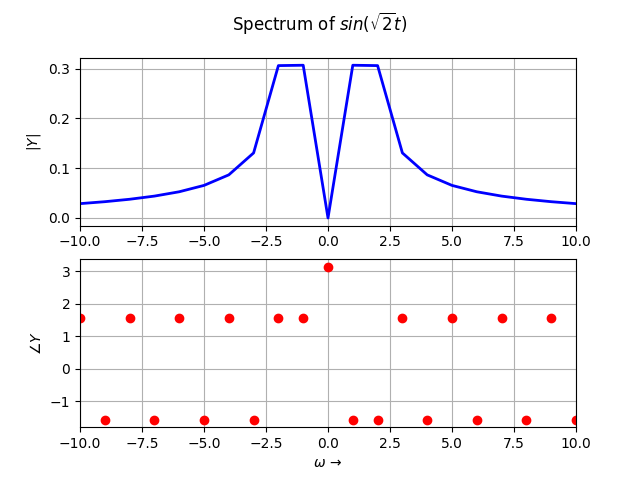
\includegraphics[scale=0.6]{Figure_0.png}
            \caption{Spectrum of $sin(\sqrt{2}t)$ without windowing}
            \label{fig:Fig1}
        \end{figure}
\subsection{With Hamming Window:}
\begin{itemize}
    \item Let us plot the DFT of $sin(\sqrt{2}t)$ with the hamming window.
    \item The following Python code does this function
\end{itemize}
    \lstset{language=Python}
    \lstset{label={lst:code_direct}}
    \lstset{basicstyle=\footnotesize}
    \begin{lstlisting}
t= np.linspace(-4*np.pi, 4*np.pi, 257);t=t[:-1]     
dt= t[1]-t[0]; fmax= 1/dt
n= np.arange(256)
wnd= fft.fftshift(0.54+0.46*np.cos(2*np.pi*n/(n.size-1)))       #Hamming Window
y= np.sin(np.sqrt(2)*t)
y= y*wnd
y[0]= 0
y= fft.fftshift(y)
Y = fft.fftshift(fft.fft(y))/256.0
w = np.linspace(-np.pi*fmax, np.pi*fmax, 257);w= w[:-1]
spectrum_plot(w,Y,r"Spectrum of $sin(\sqrt{2}t) * w(t)$",magStyle='b-o',xLimit=[-4, 4])
    \end{lstlisting}
     The obtained spectrum is as follows:
            \begin{figure}[H]
            \centering
            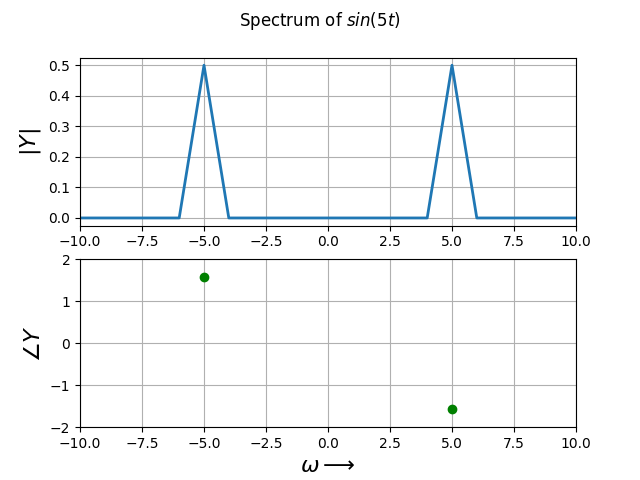
\includegraphics[scale=0.6]{Figure_1.png}
            \caption{Spectrum of $sin(\sqrt{2}t)$ with windowing}
            \label{fig:Fig2}
        \end{figure}   
\section{DFT of $cos^3(0.86 t)$ :}
Now, we look at one more function, $cos^3(0.86 t)$. We obtain the spectrum for this function with and without a Hamming window.\newline
The obtained plots are as shown below:
            \begin{figure}[H]
            \centering
            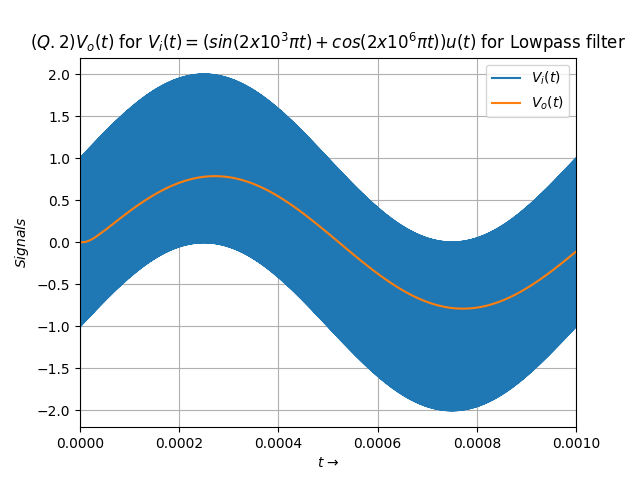
\includegraphics[scale=0.6]{Figure_2.png}
            \caption{Spectrum of $cos^3(0.86 t)$  without windowing}
            \label{fig:Fig3}
        \end{figure}
            \begin{figure}[H]
            \centering
            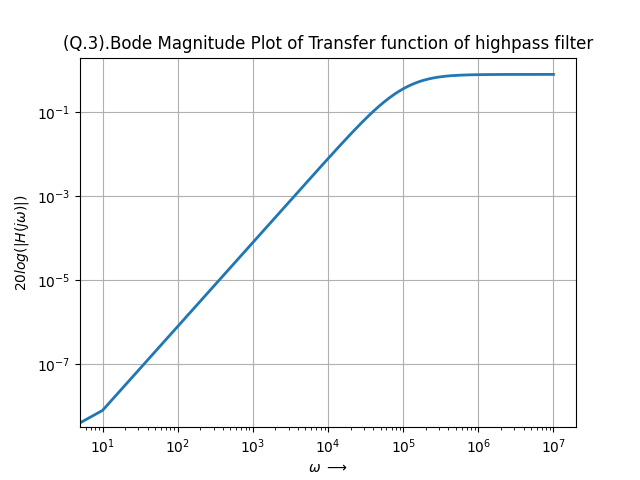
\includegraphics[scale=0.6]{Figure_3.png}
            \caption{Spectrum of $cos^3(0.86 t)$  with windowing}
            \label{fig:Fig4}
        \end{figure}
         We can see narrower and sharper peaks at the frequencies that are present in the signal.
\section{Estimating $\omega_o$ and $\delta$ from the spectrum:}
\subsection{Without noise:}
The spectrum of $cos(\omega_o t + \delta)$ with $\omega_o$= 1 and $\delta$= $\pi/4$ is as follows:
            \begin{figure}[H]
            \centering
            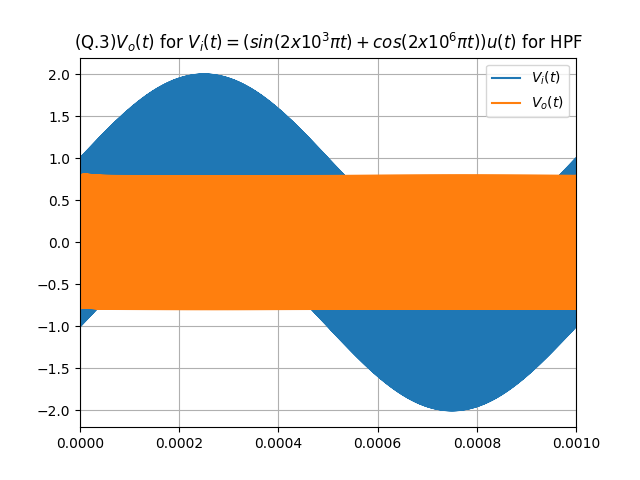
\includegraphics[scale=0.55]{Figure_4.png}
            \caption{Spectrum of $cos(\omega_o t + \delta)$  with windowing}
            \label{fig:Fig5}
        \end{figure}
After plotting the spectrum for $cos(\omega_o t + \delta)$ with $\omega_o$= 1 and $\delta$= $\pi/4$, we can see that extracting the values of $\omega_o$ and $\delta$ will not be accurate because the resolution of the frequency axis is not sufficient.\newline
So, we find the value of $\omega_o$ by using \texttt{weighted mean}.
    
    \begin{gather*}
        \omega_{o_{est}} = \frac{\sum_{\omega}|Y(j\omega)|^2\cdot \omega}{\sum_{\omega}|Y(j\omega)|^2} \forall \omega > 0
    \end{gather*}

$\delta$ can be found by calculating the phase of the DFT at $\omega$
nearest to the estimated $omega_o$ using the above method.\newline
The python code to perform the estimation part is given below:
    \lstset{language=Python}
    \lstset{label={lst:code_direct}}
    \lstset{basicstyle=\footnotesize}
    \begin{lstlisting}
#Estimation of wo & d
wo_estim= np.sum((np.abs(Y)**2*np.abs(w))/(np.sum(abs(Y)**2)))      
i= np.abs(w-wo_estim).argmin()         
d_estim= np.angle(Y[i]) 
    \end{lstlisting}
    \textbf{Estimated values:}
    \begin{itemize}
        \item Estimated value of $\omega_o$ : 0.9973353652918199
        \item Estimated value of $\delta$   : 0.7888010081342315
    \end{itemize}
    The results obtained are fairly accurate.
\subsection{With noise:}
Now, we add \texttt{white gaussian noise} to the same signal given above. We use the \texttt{randn()} function to generate the noise given by \texttt{0.1*randn(N)}, where N is the number of samples. The spectrum is as given below:
            \begin{figure}[H]
            \centering
            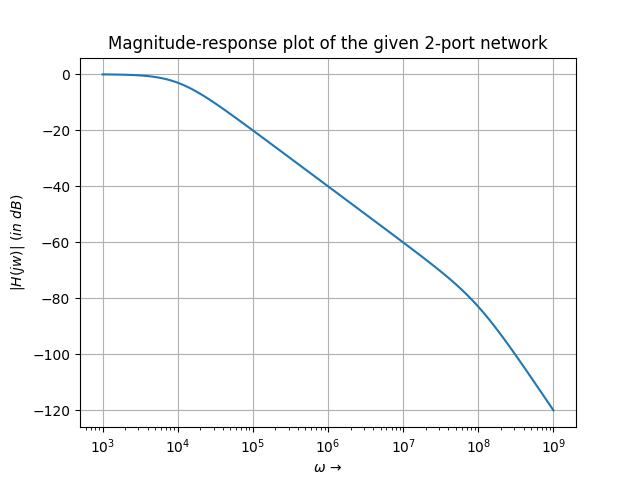
\includegraphics[scale=0.55]{Figure_5.png}
            \caption{Spectrum of $cos(\omega_o t + \delta)$  with noise}
            \label{fig:Fig6}
        \end{figure}
    We use the same method for obtaining the estimated values of $\omega_o and \delta$ .
        \textbf{Estimated values:}
    \begin{itemize}
        \item Estimated value of $\omega_o$ : 1.6477300472784084
        \item Estimated value of $\delta$   : 0.787591957607207
    \end{itemize}
    The results obtained are slightly inaccurate when compared to the case with no noise added. 
\section{DFT of Chirped Signal:}
\begin{itemize}
    \item We will plot the DFT of the function $cos(16t(1.5 + \frac{t}{2\pi}))$ where $-\pi\le t <\pi$ in 1024 steps. This signal is known as a chirped signal.
    \item the signal's frequency continuously changes from 16 to 32 radians per second. This also means that the period is 64 samples near $-\pi$ and is 32 samples near $\pi$.
\end{itemize}
The spectrum of the Chirped signal is as shown below:
            \begin{figure}[H]
            \centering
            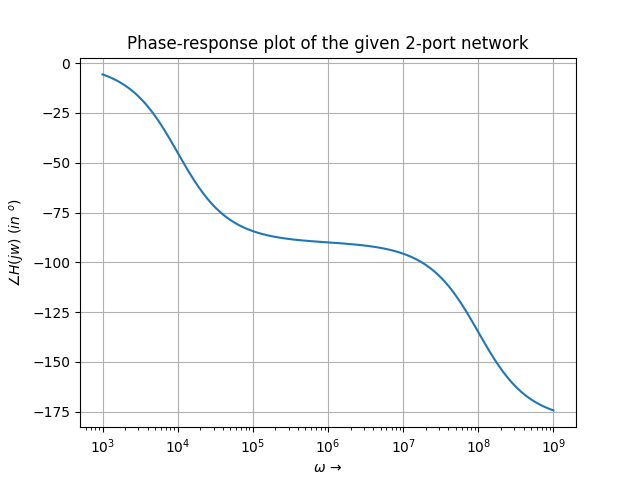
\includegraphics[scale=0.55]{Figure_6.png}
            \caption{Spectrum of chirped signal with windowing}
            \label{fig:Fig7}
        \end{figure}
Now, we break the same signal into pieces that are 64 samples wide, and calculate the DFT for each of the piece and store them as columns in 2-D array.\newline
We then plot the 2-D array as a surface plot to show how the frequency of the signal varies with time. The below Python code does the discussed function:
    \lstset{language=Python}
    \lstset{label={lst:code_direct}}
    \lstset{basicstyle=\footnotesize}
    \begin{lstlisting}
#Question 6: Variation of frequency of the above signal with time.
y_piece = np.split(y, 1024//64)         #breaking the signal into pieces
X = np.zeros((1024//64, 64), dtype=complex)     
for i in range(1024//64):           #Finding DFT for the split signal
    X[i] = fft.fftshift(fft.fft(y_piece[i]))/64

t = t[::64]     #Surface plot of the 2D array containing the DFT of each piece
w = np.linspace(-fmax*np.pi, fmax*np.pi, 65);w=w[:-1]
t, w = np.meshgrid(t, w)
fig = plt.figure(fig_no)
ax = fig.add_subplot(111, projection='3d')
surface = ax.plot_surface(w, t, abs(X).T, cmap='jet')
fig.colorbar(surface)
plt.xlabel(r"Frequency $\to$")
plt.ylabel(r"Time $\to$")
plt.title(r"Magnitude $\|Y\|$")
plt.show()
    \end{lstlisting}
    The obtained surface plot is given below:
         \begin{figure}[H]
            \centering
            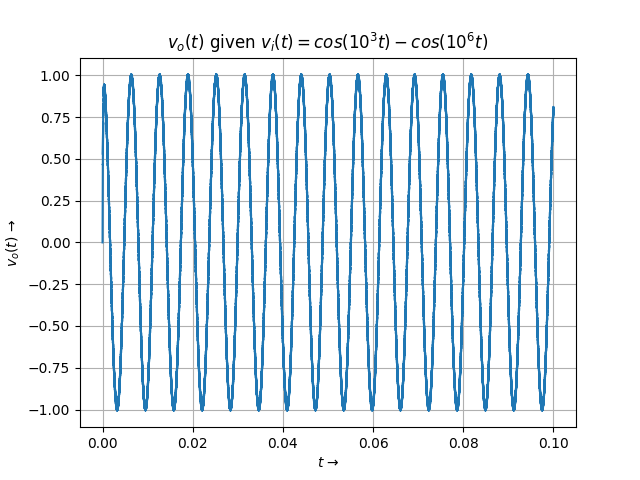
\includegraphics[scale=0.55]{Figure_7.png}
            \caption{Surface plot of spectrum of chirped signal}
            \label{fig:Fig8}
        \end{figure}
\section{Conclusion:}
In this assignment,
\begin{enumerate}
    \item we obtained the DFT of non-periodic function.
    \item we saw how the usage of Hamming window improved the results
    \item we extracted the signal parameters from the spectrum of signals
    \item we plotted the surface plot of the chirped signal to show the time dependence of frequency of the signal.
\end{enumerate}
\end{document}


